\chapter{RTS AI: \textit{StarCraft: Broodwar}}
\chaptertoc

\begin{quotation}\textit{
lala}
\\
truc
\end{quotation}

\section{How does the game work}

\subsection{RTS Gameplay}
We first introduce the basic components of a real-time strategy (RTS) game. The player is usually referred as the ``commander'' and perceives the world in an allocentric ``God's view'', performing mouse and keyboard actions to give orders to units (or squads of units) within a circumvented area (the ``map''). In a RTS, players need to gather resources to build military units and defeat their opponents. To that end, they often have \textit{worker units} (or extraction structures) than can gather resources needed to build \textit{workers}, \textit{buildings}, \textit{military units} and \textit{research upgrades}. Workers are often also builders (as in StarCraft) and are weak in fights compared to military units. Resources may have different uses, for instance in StarCraft: minerals are used for everything, whereas gas is only required for advanced buildings or military units, and technology upgrades. Buildings and research upgrades define technology trees (directed acyclic graphs) and each state of a 
\newglossaryentry{techtree}{name={tech tree},description={abbreviation for ``technological tree'', state of the technology (buildings, researches, upgrades) which are unlocked/available to a given player.}}
%\newglossaryentry{techtree}{name={tech tree},description={abbr. for ``technological tree'', the state of buildings and technologies evolution (technologies which are unlocked) of a given player}}
\glos{techtree} (or \newglossaryentry{buildtree}{name={build tree},description={abbrev. for ``buildings tree'', state of the buildings (and thus production) unlocked by a player}}\glos{buildtree}) allow for different unit type production abilities and unit spells/abilities. The military units can be of different types, any combinations of ranged, casters, contact attack, zone attacks, big, small, slow, fast, invisible, flying... In the end, a central part of the gameplay is that units can have attacks and defenses that counter each others as in a soft rock-paper-scissors. 


In chronological order, RTS include (but are not limited to): Ancient Art of War, Herzog Zwei, Dune II, Warcraft, Command \& Conquer, Warcraft II, C\&C: Red Alert, Total Annihilation, Age of Empires, StarCraft, Age of Empires II, Tzar, Cossacks, Homeworld, Battle Realms, Ground Control, Spring Engine games, Warcraft III, Total War, Warhammer 40k, Sins of a Solar Empire, Supreme Commander, StarCraft II. The differences in gameplay are in the order of number, nature and gathering methods of resources; along with construction, research and production mechanics. The duration of games vary from 15 minutes for the fastest to (1-3) hours for the ones with the biggest maps and longest gameplays. We will now focus on StarCraft, which was the focus of our implementation.


\subsection{A StarCraft Game}
\textit{StarCraft} is a science-fiction RTS game released by Blizzard Entertainment$^{TM}$ in March 1998. It was quickly expanded into \textit{StarCraft: Brood War} (SC: BW) in November 1998. In the following, when referring to StarCraft, we mean StarCraft with the Brood War expansion. StarCraft is a canonical RTS game in the sense that it helped define the genre and most gameplay mechanics seen in other RTS games are present in StarCraft. It is as much based on strategy than tactics, by opposition to the Age of Empires and Total Annihilation series. In the following of the thesis, we will focus on duel mode, also known as 1 vs. 1 (1v1). Team-play (2v2 and higher) and ``free for all'' are very interesting but were not studied in the framework of this research. These game modes particularly add a layer of coordination and bluff respectively.


StarCraft sold 9.5 millions licenses worldwide, 4.5 millions in South Korea alone \citep{StarCraftNumbers}, and reigned on competitive RTS tournaments for more than a decade. Numerous international competitions (World Cyber Games, Electronic Sports World Cup, BlizzCon, OnGameNet StarLeague, MBCGame StarLeague) and professional gaming (mainly in South Korea \citep{Chee05}) produced a massive amount of data of highly skilled human players. In South Korea, there are two TV channels dedicated to broadcasting competitive video games, particularly StarCraft. The average salary of a \glos{pro-gamer} there was up to 4 times the average South Korean salary \citep{MYMPGM} (up to \$200,000/year on contract for NaDa). Professional gamers perform about 300 actions (mouse and keyboard clicks) per minute while following and adapting their strategies, while their hearts reach 160 beats per minute (BPM are displayed live in some tournaments). StarCraft II is currently (2012) taking over StarCraft in competitive gaming but a) there is still a strong pool of highly skilled StarCraft players and b) StarCraft II has a really similar gameplay.


StarCraft (like most RTS) has a \textit{\glos{replay}} mechanism, which enables to record every player's actions such that the state of the game can be deterministically re-simulated. The only piece of stochasticity comes from ``attack miss rates'' ($\approx 47\%$) when a unit is on a lower ground than its target. These randomness generator seed is saved along with the actions in the replay. All high level players use this feature heavily either to improve their play or study opponents' styles. Observing replays allows player to see what happened under the \glos{fogofwar}, so that they can understand timing of technologies and attacks, and find clues/evidences leading to infer the strategy as well as weak points.


In StarCraft, there are three factions with very different units and technology trees:
\begin{itemize}
    \item \textit{Terran}: humans with strong defensive capabilities and balanced, averagely priced biological and mechanical units.
    \item \textit{Protoss}: advanced psionic aliens with expensive, slow to produce but resistant units.
    \item \textit{Zerg}: insectoid alien race with cheap, quick to produce but weak units.
\end{itemize}
All factions use workers to gather resources, and all other characteristics are different: from military units to ``\gloss{techtree}'', gameplay styles. Races are so different that highly skilled players focus on playing with a single race. There are two types of resources, often located close together, minerals and gas. From minerals, one can build basic buildings and units, which opens the path to more advanced buildings, technologies and units, which will in turn all require gas to be produced. While minerals can be gathered at an increasing rate (bounded asymptotically) the more workers are put at work, the gas gathering rate is quickly limited to 3 workers per gas geyser (i.e. per base).


\newglossaryentry{opening}{name=opening,description={in Chess as in RTS games: the first strategic moves of the game, the strategy of the early game},plural=openings}
\newglossaryentry{buildorder}{name=build order,description={a formal specification of timings (most often indexed on total population count) at which to perform build actions in the early game.}}
To reach a competitive amateur level, players have to study \gloss{opening} and hone their \gloss{buildorder}.


\begin{figure}[!ht]
\begin{center}
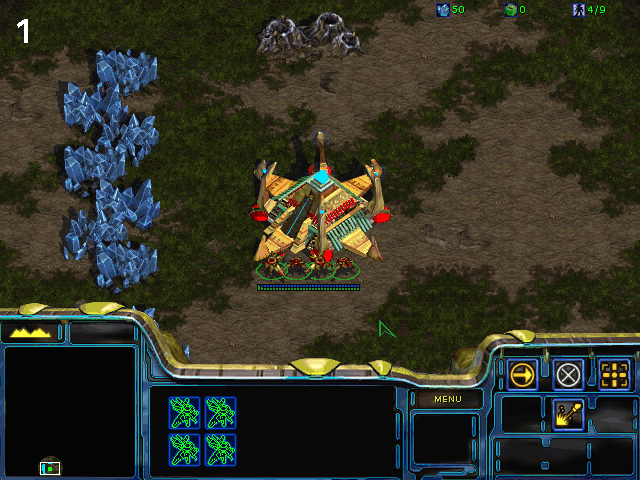
\includegraphics[width=7.8cm]{images/SC_game/SC_start_game.png}
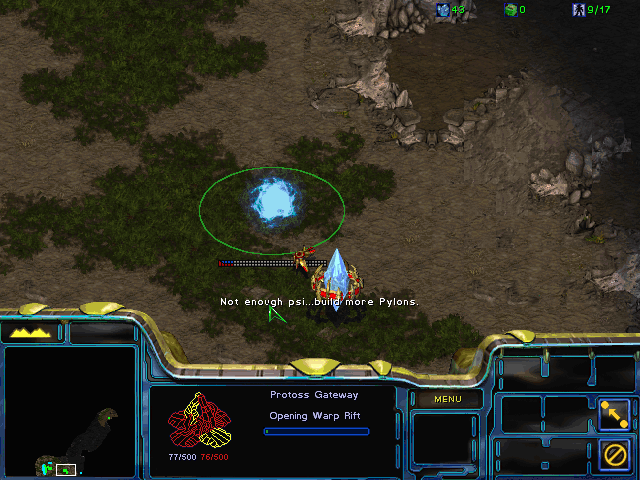
\includegraphics[width=7.8cm]{images/SC_game/SC_first_gate.png}
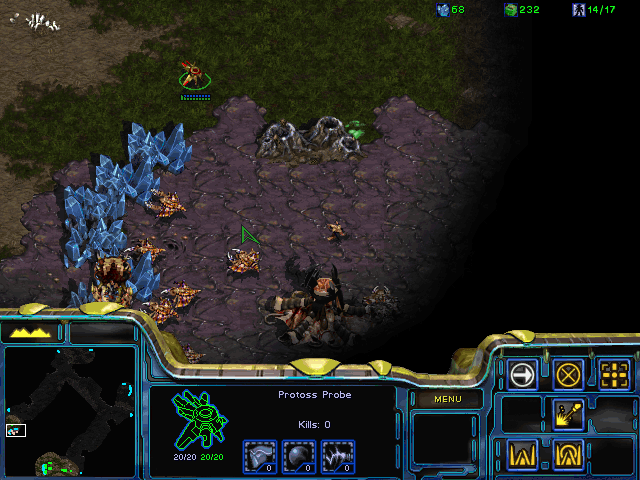
\includegraphics[width=7.8cm]{images/SC_game/SC_scout_opponent.png}
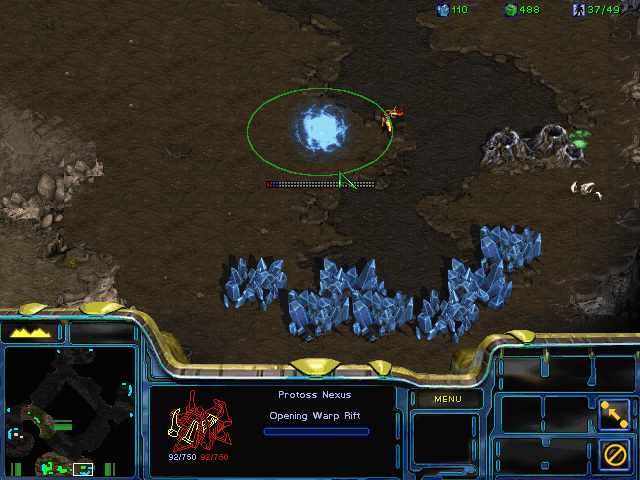
\includegraphics[width=7.8cm]{images/SC_game/SC_expand.png}
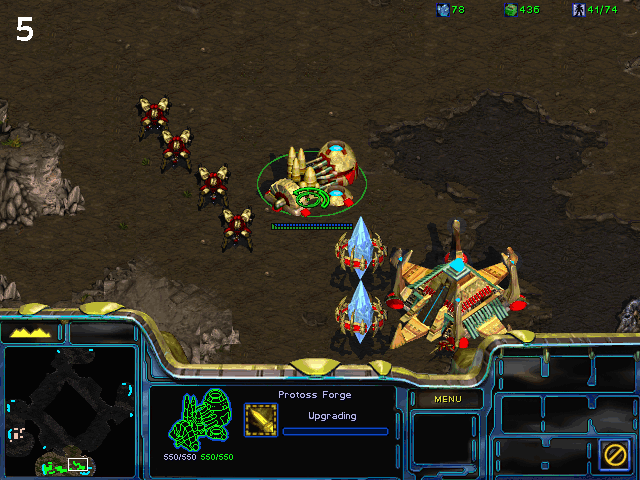
\includegraphics[width=7.8cm]{images/SC_game/SC_upgrade_attack.png}
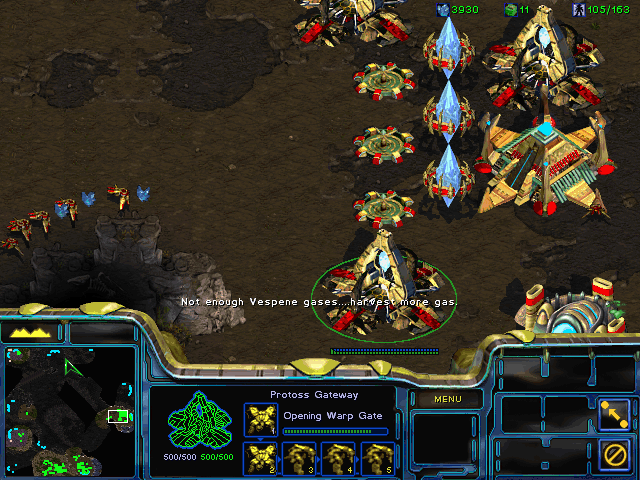
\includegraphics[width=7.8cm]{images/SC_game/SC_queue_production.png}
%SC_first_pylon.png
\label{fig:SC_game1}
\caption{Start and economical parts of a StarCraft game. The order of the screenshots goes from left to right and from top to bottom.}
\end{center}
\end{figure}

\begin{figure}[!ht]
\begin{center}
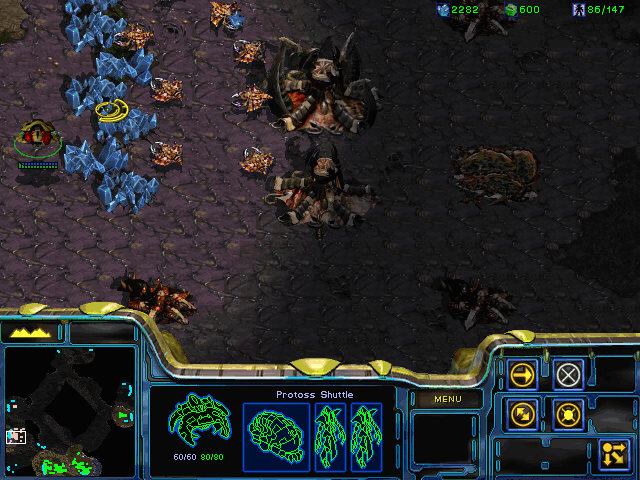
\includegraphics[width=7.8cm]{images/SC_game/SC_drop2a.png}
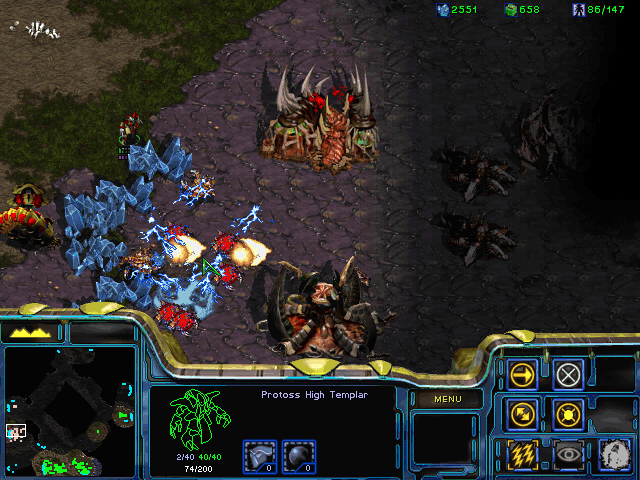
\includegraphics[width=7.8cm]{images/SC_game/SC_drop2b.png}
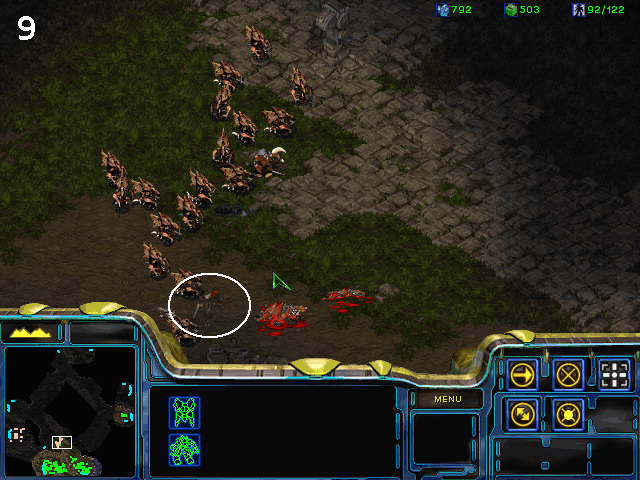
\includegraphics[width=7.8cm]{images/SC_game/SC_dt_army.png}
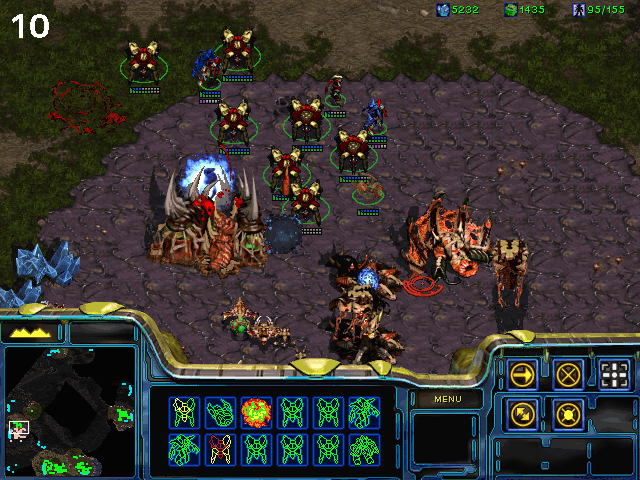
\includegraphics[width=7.8cm]{images/SC_game/SC_final_attack.png}
\label{fig:SC_game2}
\caption{Military moves from a StarCraft (PvT) game. The order of the screenshots goes from left to right and from top to bottom.}
\end{center}
\end{figure}

\section{Challenges}
In combinatorial game theory terms, competitive StarCraft is a zero sum, partial-information, deterministic strategy game.

\begin{figure}[!ht]
\begin{center}
\begin{small}
\begin{tikzpicture}
  \path[mindmap,concept color=black!80!white,text=white]
    node[concept] {RTS AI: predict, decide, perform}
    [clockwise from=-30]
    child[concept color=orange!90!black] {
      node[concept] {Micro}
      child[concept color=red!80!magenta] { node[concept] {React} }
      child { node[concept] {Optimize} }
      child[concept color=blue!30!cyan] { node[concept] {Cooperate} }
    }
    child[concept color=blue!80!black] { % TODO change color
      node[concept] {Tactics}
      child[concept color=red!80!magenta] { node[concept] {When?} }
      child { node[concept] {Where?} }
      child[concept color=blue!30!cyan] { node[concept] {How?} }
    }
    child[concept color=green!70!black] {
      node[concept] {Strategy}
      child[concept color=red!80!magenta] { node[concept] {Initiative} }
      child { node[concept] {Army composition} }
      child[concept color=blue!30!cyan] { node[concept] {Spendings balance} }
    };  
\end{tikzpicture}
\end{small}
\end{center}
\label{fig:mindmapRTS}
\caption{A mind-map of RTS AI XXX TODO}
\end{figure}

StarCraft subsumes Wargus, which has an estimated mean branching factor $1.5.10^3$ \citep{LTW} (Chess: $\approx 35$, Go: $<360$). \cite{bgweberPhD} find a branching factor of $> 1.10^6$ for StarCraft. The game complexity is roughly $10^11500$, versus the Shannon number for Chess ($10^43$).

\section{Task decomposition and linking}
\begin{figure}[!ht]
\begin{center}
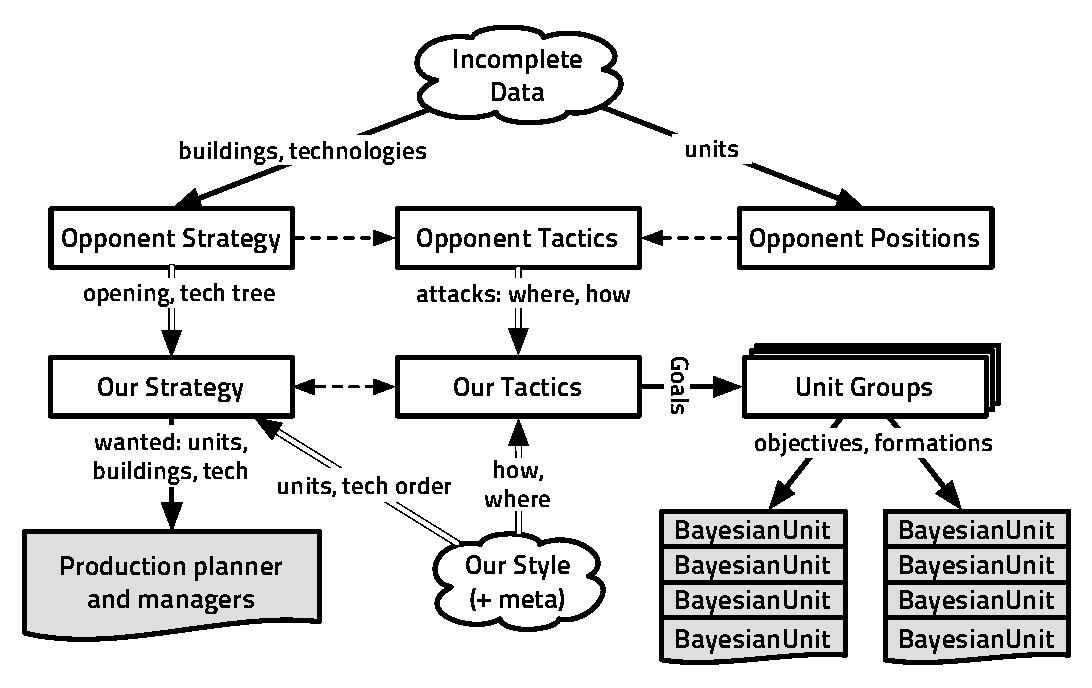
\includegraphics[width=13cm]{images/starcraft_bbq_concept.pdf}
\end{center}
\label{fig:conceptbbq}
\caption{Information-centric view of the architecture of the major components of the bot. Arrows are labeled with the information or orders they convey: dotted arrows are convey constraints, double lined arrows convey distributions, plain and simple arrows convey direct information or orders. The gray parts perform game actions (as the physical actions of the player on the keyboard and mouse).}
\end{figure}

In Fig.~\ref{fig:conceptbbq}, we present the flow of informations between the different inference and decision-making parts of the bot architecture. One can also view this problem as having a good model of one's strategy, one's opponent strategy, and taking decisions. The software architecture that we propose is to have services building and maintaining the model of the enemy as well as our state, and decision-making modules using all this information to give orders to actuators.

\begin{itemize}
\item Problem: build a real-scale software piece which is maintainable
\item State of the art: shared memories, shared states
\item Our take: we transmit distributions, states stay in modules
\item Results: XXX (atm too much state), also competitions results
\end{itemize}

% XXX 
XXX Real-time strategy (RTS) gameplay consist in producing and managing group of units with attacks and movements specificities in order to defeat an enemy. Most often, it is required to gather resources and build up an economic and military power while expanding a technology tree. Parts of the map not in the sight range of the player's units are under \textit{\glos{fogofwar}}, so the player only has partial information about the enemy buildings and army. The way by which we expand the tech tree, the specific units composing the army, and the general stance (aggressive or defensive) form what we call \textit{strategy}. At the lower level, the actions performed by the player (human or not) to optimize the effectiveness of its units is called \textit{micro-management}. In between lies \textit{tactics}: where to attack, and how. A good human player takes much data in consideration when choosing: are there flaws in the defense? Which spot is more worthy to attack? How much am I vulnerable for attacking here? Is the terrain (height, chokes) to my advantage? etc.

